\chapter{Theoretische Einführung}



\section{Grundlagen der additiven Fertigung mittels selektivem Laserschmelzen (SLM)}
	Additiv gefertigte Produkte (\emph{additive manifacturing}, kurz: \emph{AM}) aus dem
	3D-Drucker spielen in unserem Leben eine immer größere Rolle. AM bezeichnet hierbei das
	Fertigen eines Objektes durch hinzufügen von Material, während im Gegensatz dazu die
	traditionelle subtraktive Fertigung Material durch Fräsen oder ähnliches aus einem Werkstück
	entfernt. Während sich bereits ein Hobbymarkt für preisgünstige 3D-Drucker im eigenen Haushalt
	etabliert hat, ist die industrielle Anwendung nicht zu vernachlässigen. Essentium, ein
	Hersteller von industriellen 3D-Druckern und Materialien, hat eine Umfrage zur industriellen
	Nutzung von 3D-Druckern durchgeführt. Diese Umfrage ergab eine Verdopplung des Anteils von AM
	in der industriellen Produktion innerhalb eines Jahres. Während der Anteil 2018 noch bei 21 \%
	lag, änderte er sich innerhalb eines Jahres auf 40 \% \cite{stevenson2019survey}.

	Obwohl es eine Vielzahl unterschiedlicher Methoden der additiven Fertigung gibt, funktionieren
	alle nach einem ähnlichen Grundprinzip: Das digitale 3-dimension\-ale Modell wird durch einen
	sogenannten \emph{Slicer} in Schnittebenen unterteilt, die nacheinander maschinell produziert
	und aufgeschichtet werden.

	%\subsection{Funktionsweise und Unterschiede zu anderen Methoden}
	\subsection{Funktionsweise und Unterschiede zum FDM-Druck}
		Das bekannteste Verfahren zur additiven Fertigung ist das \emph{Fused Depositing Modeling}
		(\emph{FDM}), aus Markenrechtsgründen auch bekannt als \emph{Fused Filament Fabrication}
		(\emph{FFF}). Wie in Abbildung \ref{fig:fdm} dargestellt wird dabei ein Kunststofffilament
		mithilfe eines Fördermechanismuses (\emph{extruder}) durch eine heißen Düse \emph{hotend}
		geschoben und dort geschmolzen. Diese Düse ist Teil eines beweglichen Druckkopfs und fährt
		während des Extrudierens die geslicte Schnittebene ab, sodass Ebene für Ebene das
		gewünschte Objekt aufgeschichtet wird. Schichten sind bei diesem Verfahren üblicherweise
		zwischen \SI{0,025}{\milli\meter} und \SI{1,25}{\milli\meter} dick
		\cite{wikipedia2021fused}.

		\begin{figure}[!ht]
			\centering
			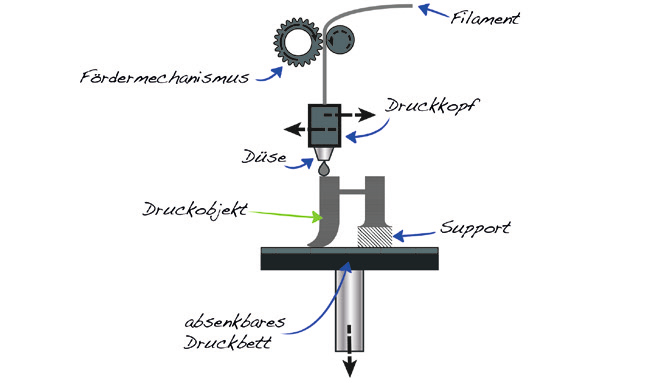
\includegraphics[width=0.9\textwidth]{chapter/main/theory/img/fdm.png}
			\caption[Schematische Darstellung des FDM-/FFF-Verfahrens]{Schematische Darstellung
			einer möglichen Konfiguration des als FDM oder FFF bekannten 3D-Druck-Verfahrens. Ein
			Fördermechanismus schiebt das Filament durch eine aufgeheizte Düse. Durch eine
			Bewegung der Düse und/oder des Druckbetts in 3 Achsen erfolgt eine Formung
			des gewünschten Objektes Ebene für Ebene. \cite{horsch20143d}}
			\label{fig:fdm}
		\end{figure}

		Obwohl dieses Verfahren relativ einfach umzusetzen ist, wird es durch verschiedene
		Faktoren limitiert. So ist beispielsweise für die Qualität des Drucks unter anderem die
		Form des zu druckenden Objekts relevant. Außerdem ist dieses Verfahren auf bestimmte
		Materialien beschränkt, wie Thermoplaste und Formwachse. Die Druckbarkeit wird nicht
		zuletzt auch durch die Gravitation beschränkt, sodass je nach Form auch Stützstrukturen
		(\emph{support}) erforderlich sein können \cite{wikipedia2021fused}.

		Das in dieser Arbeit betrachtete Verfahren ist jedoch das hauptsächlich industriell
		verwendete \emph{selektive Laserschmelzen} (\emph{SLM}). Abbildung \ref{fig:slm_sls}
		zeigt den Aufbau der nach diesem Verfahren funktionierenden Drucker. Diese bestehen
		hierbei aus zwei Gefäßen mit beweglichen Böden. Das Gefäß für den Materialvorrat
		(\emph{feed container}) ist mit dem Material in Pulverform gefüllt, während das andere
		wenig bis gar nicht gefüllt ist. Beim Drucken einer neuen Ebene hebt sich der Boden des
		Materialvorrats und eine Walze (\emph{Beschichtungseinheit}) überträgt das dosierte
		Material in den Druckraum, dessen Druckbett abgesenkt wird. Ein beweglicher Laser fährt
		nun die gewünschte Schnittebene ab und verschmilzt das Pulver zu einer festen Form
		\cite{horsch20143d}.
		%\todo[color=red]{Quelle dazu finden bzw. nennen. Florian Horsch?}

		\begin{figure}[!ht]
			\centering
			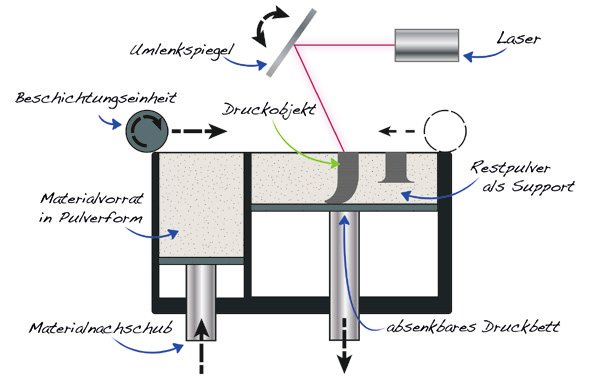
\includegraphics[width=0.9\textwidth]{chapter/main/theory/img/sls_slm.png}
			\caption[Schematische Darstellung des SLM-Verfahrens]{Schematische Darstellung des
			SLM-Verfahrens. Der bewegliche Spiegel sorgt für eine präzise Positionierung des
			Laserpunktes. Während sich der Boden des Vorrats\-gefäßes im Prozess anhebt, senkt
			sich der Boden des Druckraums ab. \cite{horsch20143d}}
			\label{fig:slm_sls}
		\end{figure}

		Das Druckbett wird üblicherweise um \SI{30}{\micro\meter} bis \SI{100}{\micro\meter}
		abgesenkt \cite{song2012effects}, wobei ferner auch dickere Schichthöhen Verwendung finden
		\cite{shi2016performance}. Zu den am häufigsten verwendeten Materialien, die beim
		SLM-Verfahren verwendet werden, zählen Titanlegierungen, insbesondere das in der Luft- und
		Raumfahrt populäre Ti6Al4V \cite{song2012effects,shi2016performance,brandl2012morphology}.
		Aluminiumlegierungen werden wegen ihrer Eignung zum Leichtbau vor allem in der
		Automobilindustrie verwendet \cite{yan2020comparative,zou2017study}.

	\subsection{Defekte in gefertigten Objekten}
		\label{subsec:defects}
		\subsubsection{Porenbildung}
		\begin{figure}[!ht]
			\centering
			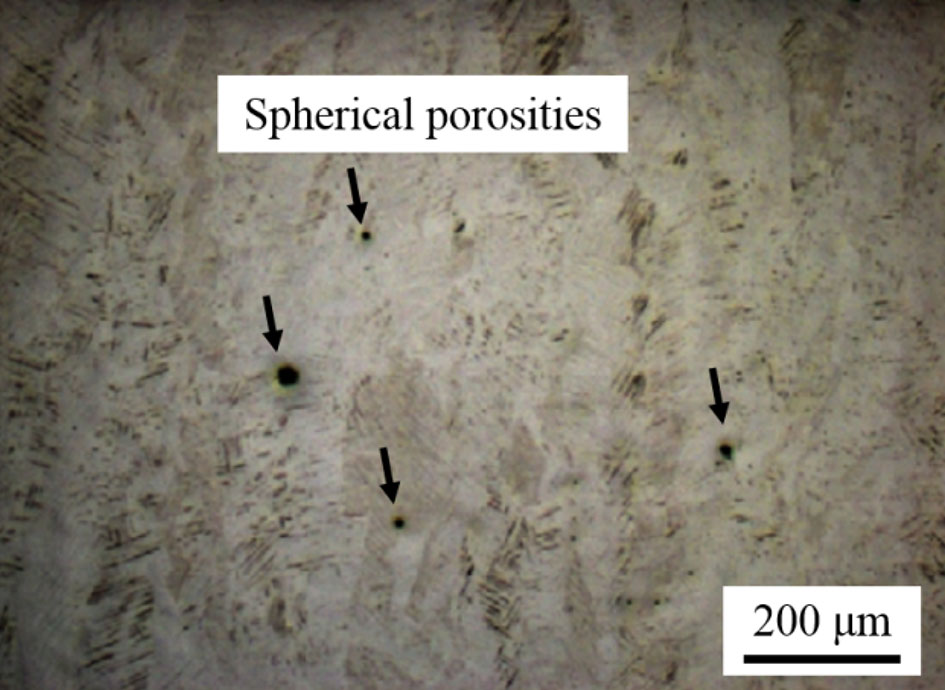
\includegraphics[width=0.6\textwidth]{chapter/main/theory/img/defects/porosities.png}
			\caption{Poren sphärischer Form unterschiedlicher Größe entstehen durch Gaseinschlüsse
			\cite{zhang2017defect}}
			\label{fig:defects_porosities}
		\end{figure}

		Aufgrund verschiedener physikalischer Phänomene treten während des Verfahrens Vorgänge
		auf, die sich in Defekten bemerkbar machen. Einer der bekanntesten Defekte ist die
		\emph{Porenbildung}. Poren sind Gaseinschlüsse und zählen mit einer Größe von weniger als
		\SI{100}{\micro\meter} zu den kleinsten der hier aufgeführten Defekten
		\cite{zhang2017defect}. Es werden zwei verschiedene Gasquellen unterschieden. Während eine
		Quelle des dafür notwendigen Gases die Verdampfung mancher Legierungsbestandteile, wie
		beispielweise Magnesium, sein kann, kann ein Gaseinschluss nicht zuletzt auch durch
		Einschluss des beim Prozess verwendeten Schutzgases erfolgen \cite{galy2018main}. Dieses
		wird zur Verhinderung von Oxidationen verwendet. In letzterem Fall kann zum Beispiel eine
		zu geringe Packungsdichte des verwendeten Materialpulvers die Ursache sein. Das Gas dringt
		hierbei während des Schmelzprozesses in die Schmelze ein, erreicht aber aufgrund einer
		hohen Kühlrate die Oberfläche nicht vor dem Erstarren, sodass beim Erhärten des Materials
		ein Gaseinschluss die Folge ist. Aus diesem Grund haben Poren eine näherungsweise
		sphärische Form. Sie sind üblicherweise im gefertigten Objekt gleichverteilt aufzufinden.

		Das komplette Eliminieren aller Poren gilt als sehr schwer \cite{zhang2017defect}.
		Galy et al. zufolge hat die Porengröße und -form einen entscheidenden Einfluss auf die
		Qualität des Endproduktes. Größere Makroporen verschlechtern die Qualität stärker als
		kleinere Mikroporen, wobei sich mehrere Mikroporen zu größeren Makroporen vereinigen
		können. Eine stärkere Entrundung der sphärischen Form der Poren kann eine Ursache von
		Rissen im Objekt sein \cite{galy2018main}. Poren unterschiedlicher Größe sind in Abbildung
		\ref{fig:defects_porosities} zu sehen.

		\subsubsection{Mangelnde Verschmelzung}
		Eine mangelnde Verschmelzung (\emph{lack-of-fusion}, kurz: \emph{LOF}) entsteht
		überwiegend durch unzureichende Energiezufuhr während des Schmelzprozesses. Ist die von
		Laser zugeführte Energie zu niedrig, vermindert sich die Breite der aufgeschmolzenen Bahn.
		Wie in Abbildung \ref{fig:defects_lof} a) zu sehen kann dies durch unzureichende
		Überlappung der Bahnen zu fehlender Haftung zwischen diesen führen (sogenannte
		\emph{bonding defects}). Außerdem resultiert die LOF in zahlreichen Pulvereinschlüssen
		(Abbildung \ref{fig:defects_lof} b)). Sollte die Energiezufuhr sogar unzureichend sein,
		um die gesamte Schichthöhe zu durchdringen, führt dies zu mangelhafter Bindung zwischen
		den Ebenen. Aus diesen Gründen sind Defekte die LOF betreffend hauptsächlich zwischen
		den Bahnen einer Ebene und zwischen den Ebenen selbst zu finden. Da diese Defekte eine
		Erhöhung der Rauheit zur Folge haben, wird der Materialfluss der nächsten Ebene ebenfalls
		gestört, sodass Zwischenebenendefekte auftreten können, die graduell durch mehrere Ebenen
		propagieren und somit Defekte zur Folge haben, die sich über mehrere Ebenen erstrecken.
		Dieser Effekt kann auch durch das Abkühlen der Oberfläche entstehen. Die damit verbundene
		verminderten Benetzbarkeit stellt auch ein Problem bei der Aneinanderbindung von Bahnen
		dar \cite{zhang2017defect}.

		\begin{figure}[!ht]
			\centering
			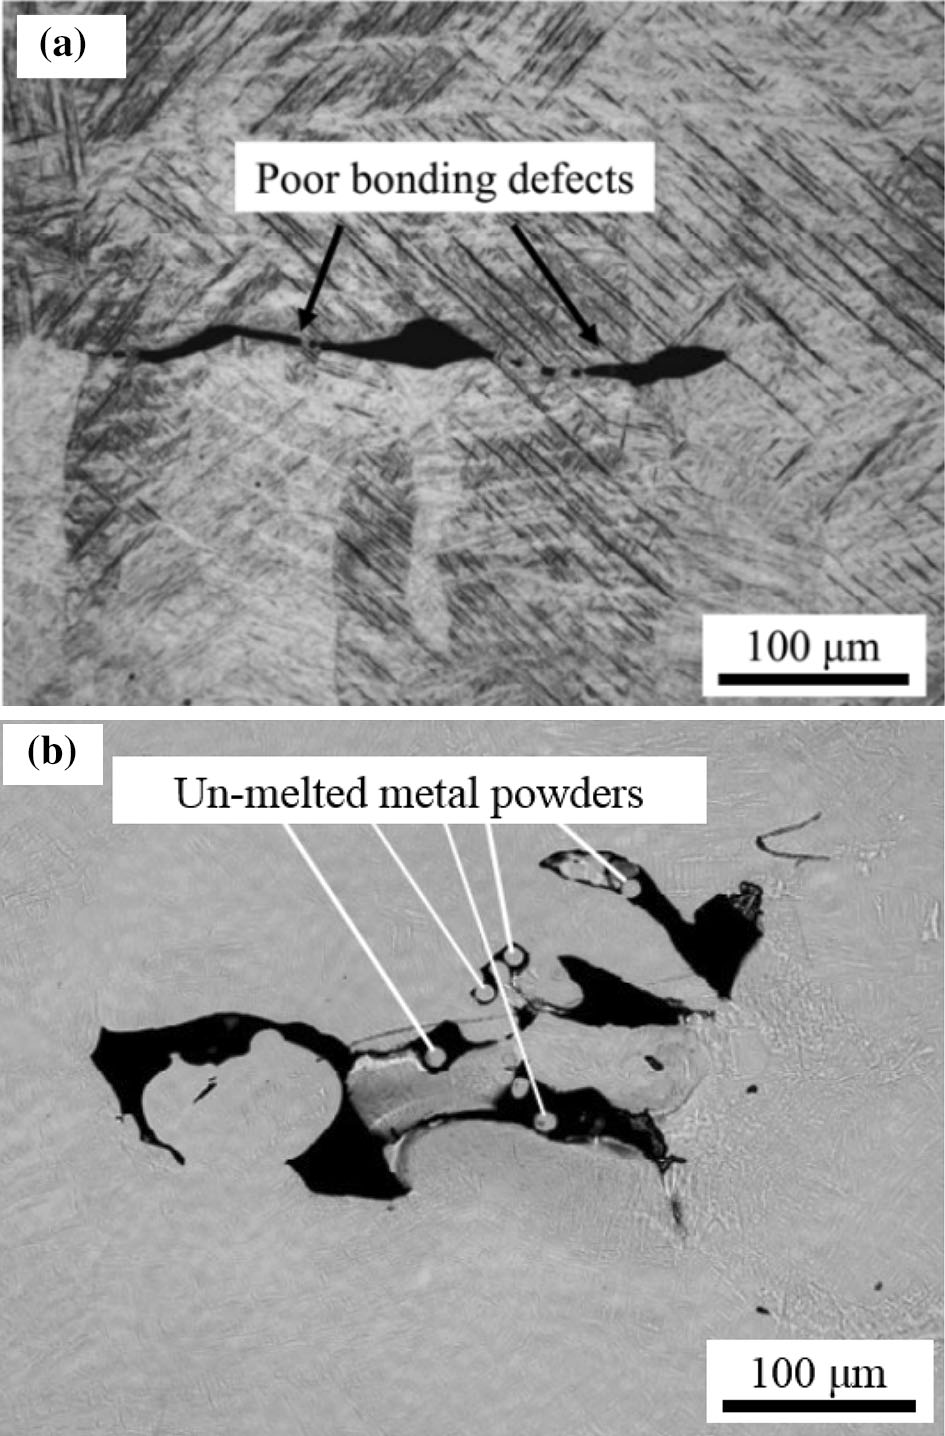
\includegraphics[width=0.6\textwidth]{chapter/main/theory/img/defects/lack_of_fusion.png}
			\caption{a) Zwei Bahnen mit schlechter Verbindung durch mangelnde Überlappung
			b) Gut erkennbare Pulvereinschlüsse durch unzureichendes Aufschmelzen des Pulvers
			in Hohlräumen \cite{zhang2017defect}}
			\label{fig:defects_lof}
		\end{figure}

		\subsubsection{Risse}
		Während des Schmelzprozesses herrschen nach dem Schmelzen Kühlraten von bis zu
		\SI{e8}{\kelvin\per\second} \cite{zhang2017defect}. Der dadurch entstehende
		Temperaturgradient und die damit verbundene unterschiedlich starke thermische
		Materialausdehnung führt zu hohen Verspannungen im Material. Diese Spannungen können nun
		dafür sorgen, dass Risse (\emph{cracks}) entstehen und dass diese weiter durch das
		Material propagieren. Abbildung \ref{fig:defects_cracks} zeigt verschiedene Stellen eines
		Risses, der sich an einer Oberfläche gebildet hat und weiter in das gefertigte Objekt
		hineinpropagiert ist \cite{zhang2017defect}. Wie bereits in Abschnitt \emph{Porenbildung}
		erwähnt können auch nicht-sphärische Poren besonders begünstigend auf die Rissbildung wirken
		\cite{galy2018main}.

		\begin{figure}[!ht]
			\centering
			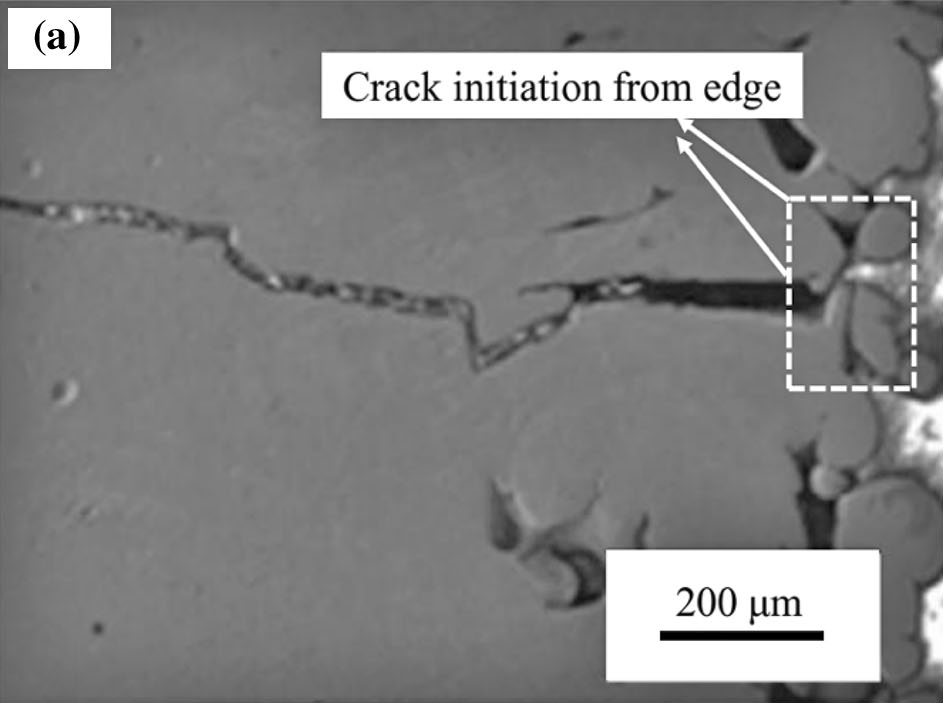
\includegraphics[width=0.6\textwidth]{chapter/main/theory/img/defects/cracks_part.png}
			\caption{Aufnahme des Rands eines produzierten Objektes, von dem ein Riss ausgeht. Es
			ist gut erkennbar wie der Riss von Rand ausgehen in das Objekt hineinpropagiert ist.
			\cite{zhang2017defect}}
			\label{fig:defects_cracks}
		\end{figure}

		\subsubsection{Keyhole-Effekte}
		In Abbildung \ref{fig:defects_keyholes} ist eine starke Änderung in der Form des
		verfestigten Materials zu sehen. Anstatt eines flachen und breiten Querschnitts ist hier
		das Resultat eines schmalen und tiefen V-förmigen Schmelzbades zu sehen. Dieser Effekt
		tritt besonders bei hohen Temperaturen auf. In diesem Fall vaporisiert ein Teil des
		Materials. Der entstehende Dampf verdrängt das umliegende geschmolzene Material teilweise,
		sodass sich eine Dampfkapillare ausbildet. Das geschmolzene Material umfließt diese und
		erstarrt hinter ihr. Dieser Effekt wird \emph{Keyhole-Effekte} genannt.

		\begin{figure}[!ht]
			\centering
			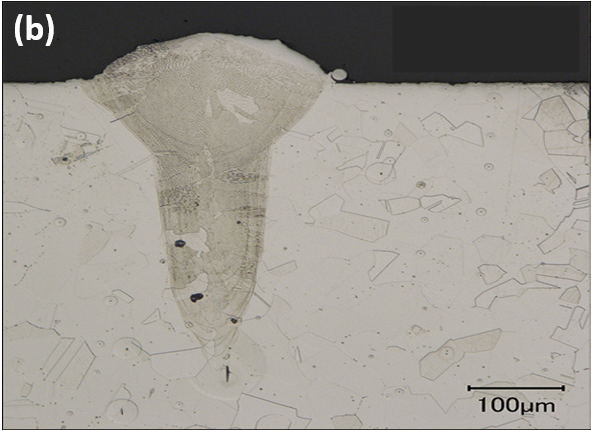
\includegraphics[width=0.6\textwidth]{chapter/main/theory/img/defects/keyhole.png}
			\caption{Ein druch den Keyhole entstandener Defekt \cite{eskandarisabzi2019defect}}
			\label{fig:defects_keyholes}
		\end{figure}

	\subsection{Wichtige Parameter und Einfluss der Lasergeschwindigkeit}
		Beim SLM-Verfahren sind verschiedene Parameter einstellbar, die das Resultat in
		unterschiedlicher Weise und Stärke beeinflussen. Eine kategorische Übersicht über alle
		beim SLM-Prozess variierbaren Parameter ist in Abbildung \ref{fig:scheme_parameters} zu
		finden.

		\begin{figure}[!ht]
			\centering
			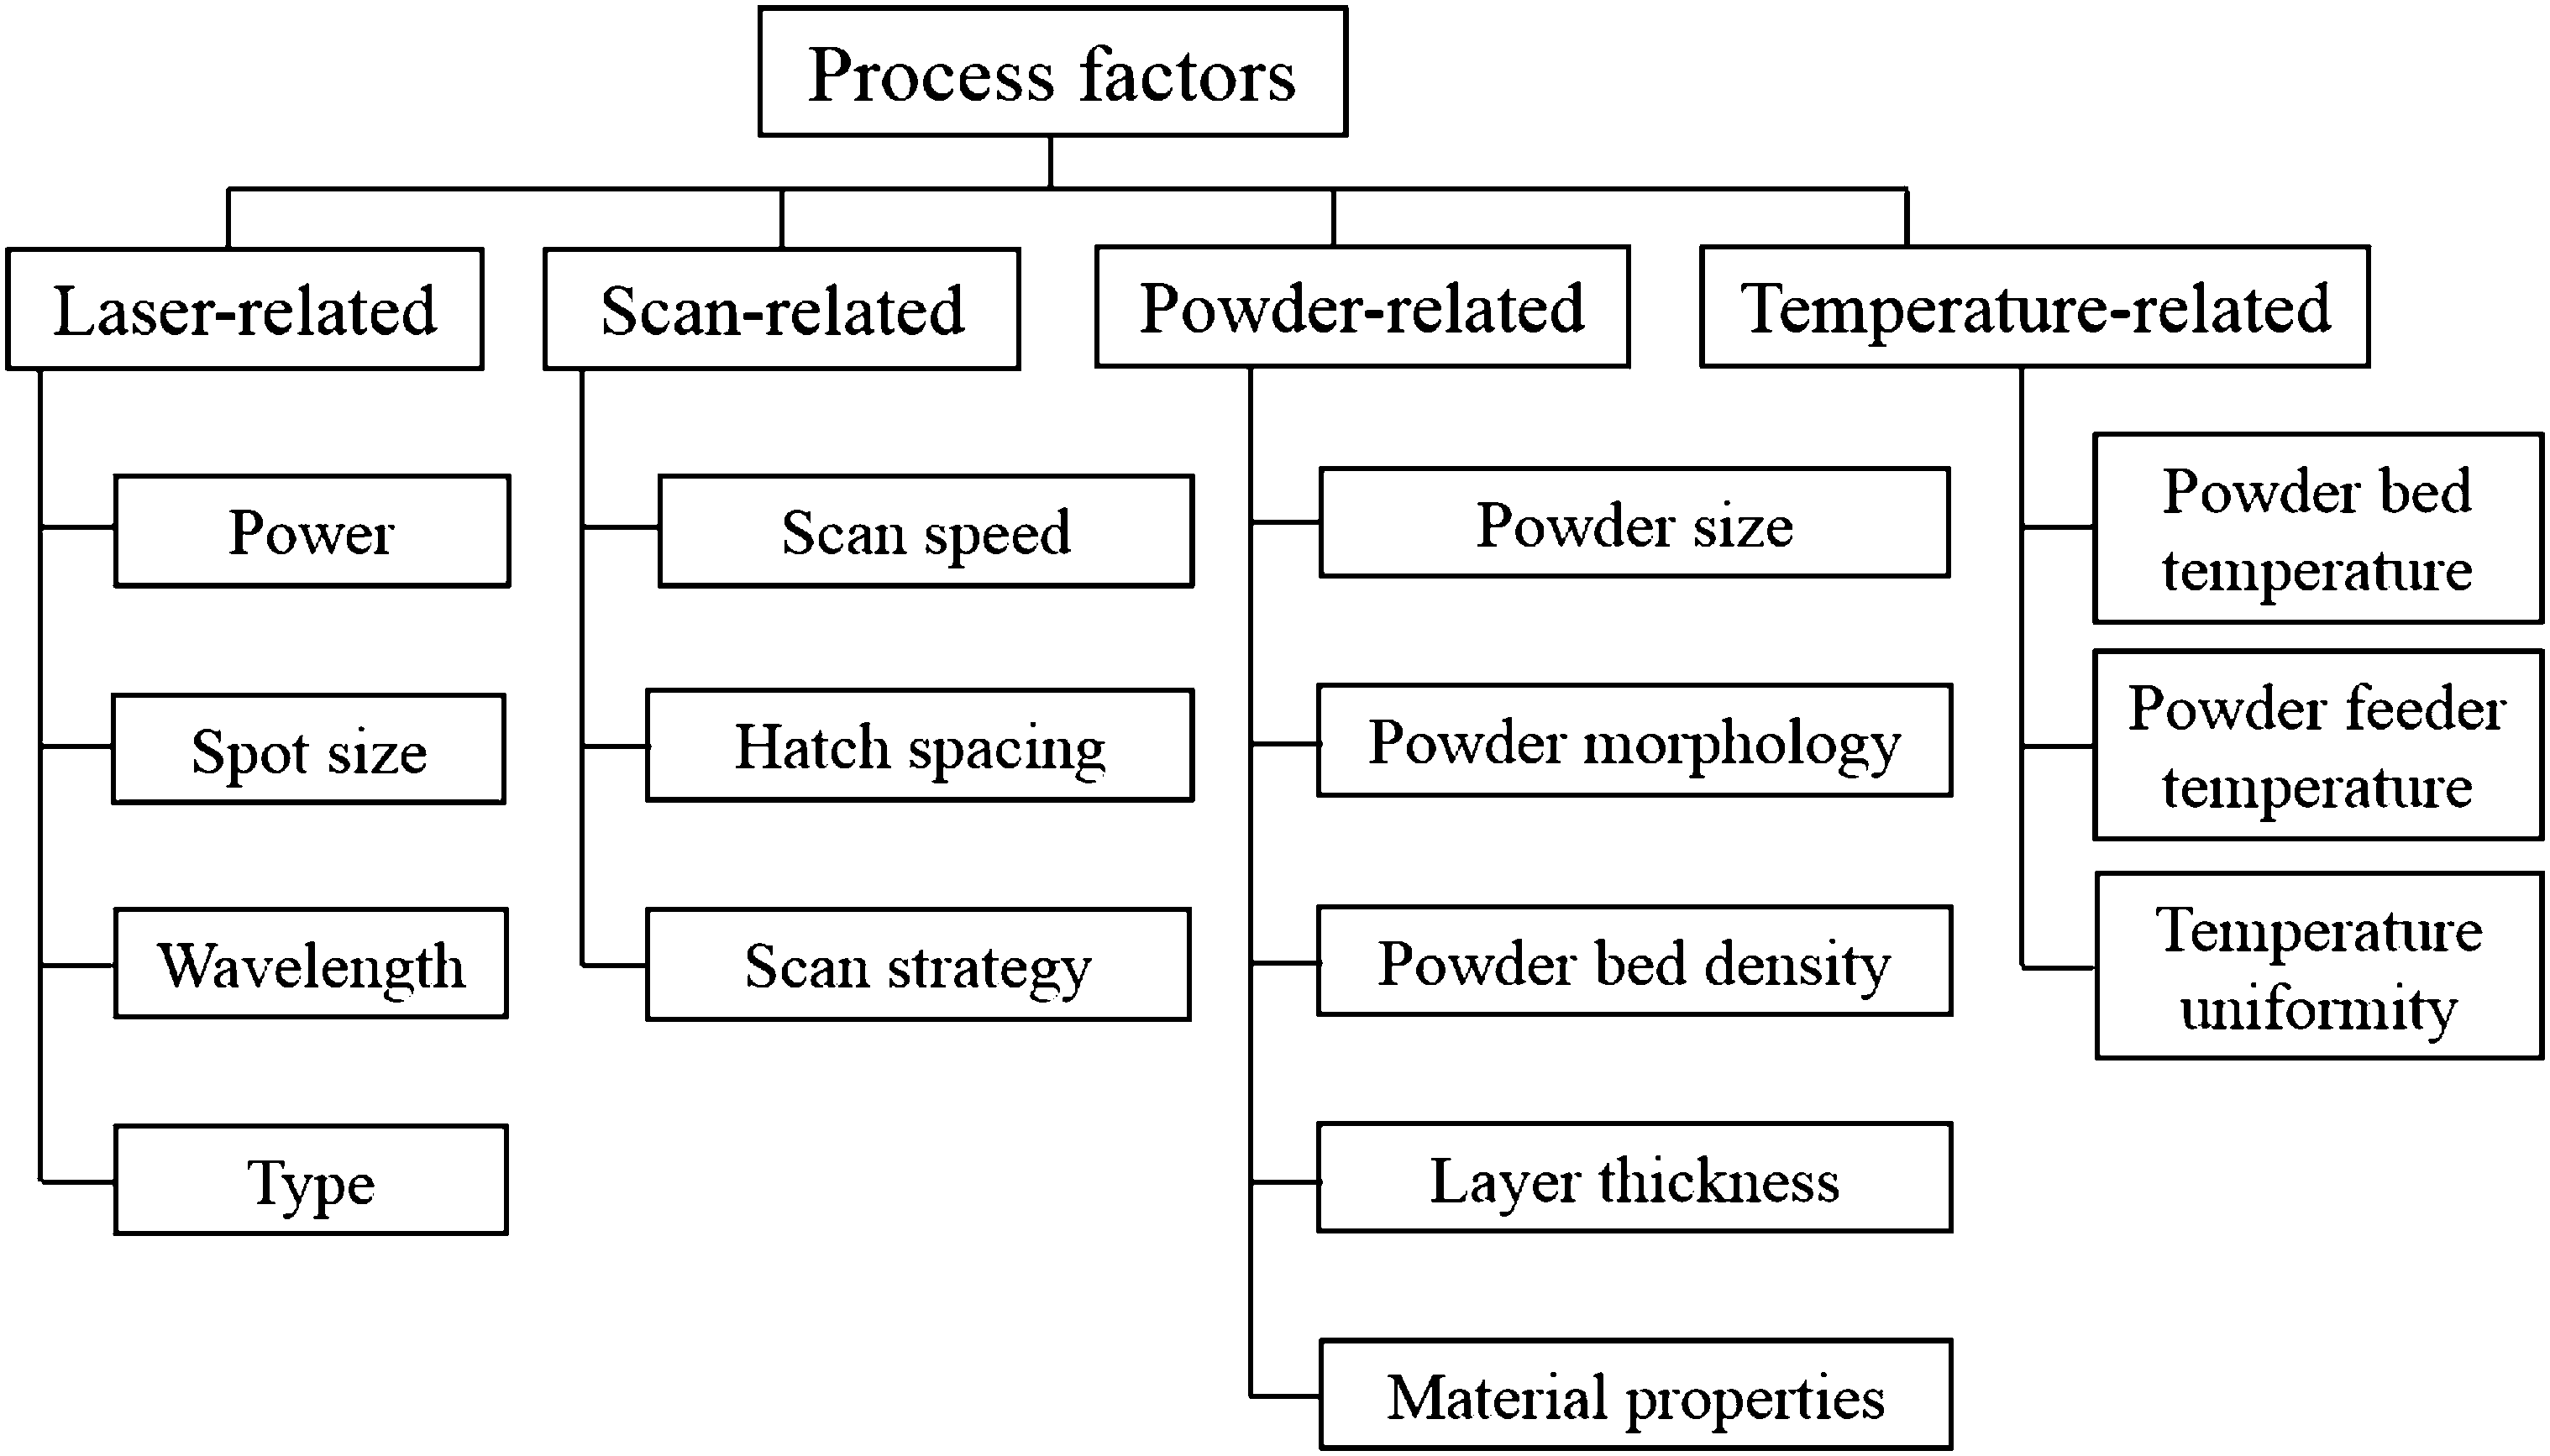
\includegraphics[width=0.9\textwidth]{chapter/main/theory/img/scheme_parameters_2.png}
			\caption{Eine Übersicht aller beim SLM-Verfahren einstellbaren Parameter nach
			Kategorie geordnet \cite{zhang2017defect,aboulkhair2014reducing}}
			\label{fig:scheme_parameters}
		\end{figure}

		Aufgrund der in Abschnitt \ref{subsec:defects} angesprochenen Defekte ist es beim
		SLM wichtig das Pulver zwar komplett zu schmelzen, aber nicht zu viel Energie zuzuführen.
		Variierbare Parameter, die das besonders stark beeinflussen, sind die Lasergeschwindigkeit
		(\emph{scanning speed}), die Laserleistung, der horizontale Bahnabstand
		(\emph{hatch distance} oder \emph{hatch spacing}), die Wellenlänge des Lasers, der
		Durchmesser des fokussierten Laserpunktes (\emph{spot size}) und die durch die Dicke der
		Pulverschicht bestimmte  Schichtdicke (\emph{layer thickness}) \cite{sadali2020influence}.
		Abbildung \ref{fig:slm_parameters} zeigt die räumliche Einordnun dieser Parameter. Da für
		diese Arbeit die Größenordnung im Bereich der einzelnen Pulverpartikel von Interesse ist,
		werden im weiteren Verlauf der Bahnabstand und die Schichtdicke nicht weiter betrachtet.

		\begin{figure}[!ht]
			\centering
			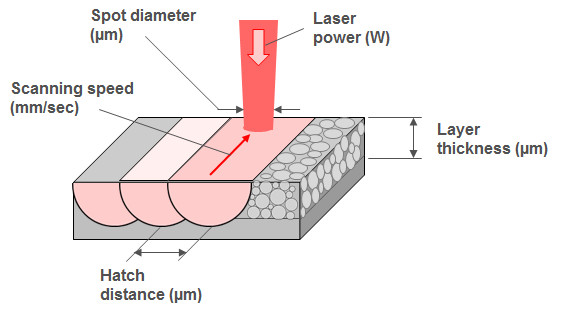
\includegraphics[width=0.9\textwidth]{chapter/main/theory/img/slm_parameters.jpg}
			\caption{Darstellung und räumliche Einordnung der wichtigsten einstellbaren Parameter
			beim SLM-Druck und ihre üblichen Größenordnungen \cite{saunders2017x}}
			\label{fig:slm_parameters}
		\end{figure}

		Für ein optimales Ergebnis bedarf es natürlich einer optimalen Abstimmung der Parameter
		aufeinander. Beispielsweise ist für eine Erhöhung der Lasergeschwindigkeit oft eine
		größere Laserleistung nötig, um das Schmelzen des Materials weiterhin gewährleisten
		zu können.

		Sadali et al. beobachteten, dass mit steigender Lasergeschwindigkeit die Größe der Poren
		reduziert wird. Außerdem entstehen weniger Spritzer (\emph{splashing effect}).
		Kugelförmige Materialanhäufungen auf der Oberfläche, die bei der Auftrennung von
		instabilen Flüssigspuren durch mangelnde Benetzbarkeit entstehen können
		(\emph{balling effect}), werden mit steigender Geschwindigkeit nicht nur weniger, sondern
		auch kleiner. Abbildung \ref{fig:defects_balling} zeigt eine Oberfläche, auf der der
		\emph{balling effect} auftritt. Diese Ballförmigen Anhäufungen können auch in Clustern
		auftreten.

		Nichtsdestotrotz bedeutet dies nicht unbedingt, dass ein schnellerer Laser grundsätzlich
		ein besseres Gesamtergebnis erzielt. Mit höherer Geschwindigkeit treten beispielsweise
		auch mehr Mikrorisse auf. Während diese durch \emph{Heißisostatisches Pressen}
		(\emph{HIP}) zwar minimiert werden können, treten ab einer gewissen Geschwindigkeit jedoch
		vermehrt unnerwünschte Effekte auf, deren nachträgliche Reduktion durch HIP nicht möglich
		ist \cite{sadali2020influence}.

		\begin{figure}[!ht]
			\centering
			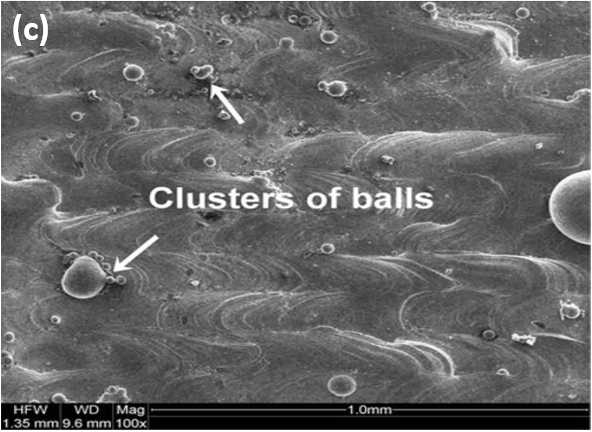
\includegraphics[width=0.7\textwidth]{chapter/main/theory/img/defects/balling.png}
			\caption{Der sogenannte \emph{balling effect} entsteht, wenn die Benetzbarkeit der
			darunter liegenden Schicht nicht ausreicht, sodass sich aus dem geschmolzenen
			Material kugelförmige Ansammlungen bilden \cite{eskandarisabzi2019defect}}
			\label{fig:defects_balling}
		\end{figure}


\section{Molekulardynamische Modellierung von SLM}
	\subsection{Grundlegende Funktionsweise der Molekulardynamiksimulation (MD)}
		Um ein System vieler Teilchen zu betrachten bedarf es eines Modell. Mithilfe einer
		\emph{Molekulardynamiksimulation} (\emph{MD}) geschieht diese Betrachtung atomistisch.
		Das bedeutet, dass die Teilchen einzeln betrachtet und als fundamentale, nicht teilbare
		Atome angesehen werden. Um die Trajektorien aller Teilchen in einem System großer
		Teilchenzahl $N$ zu bestimmen, bedarf es der Lösung der zugehörigen Bewegungsgleichungen

		\begin{align}
			m_i \ddot{\uvec{x}}_i &= \uvec{F}_i
			& \text{mit} &&
			\uvec{F}_{i} &= \sum_{\substack{j=0\\j \neq i}}^{N-1} \uvec{F}_{ij}
			= -\sum_{\substack{j=0\\j \neq i}}^{N-1} \nabla_i U_j = -\nabla_i U
			\label{eq:newtone_dgl}
			.
		\end{align}

		Hierbei ist $m_i$ die Masse des Teilchens $i$, $\uvec{x}_i$ der Ortsvektor von diesem und
		$\uvec{F}_{i}$ die vektorielle Gesamtkraft auf dieses. Weiterhin ist $\uvec{F}_{ij}$ die
		Einzelkraft zwischen zwei Teilchen $i$ und $j$ sowie $U_i$ das vom Teilchen $i$ ausgehende
		Potential und $\nabla_i$ der Gradient in der Koordinate $\uvec{x}_i$. Da diese
		Bewegungsgleichungen für Teilchenzahlen $N \geq 3$ im Allgemeinen nicht analytisch lösbar
		sind, %\todo[color=green]{Bezug auf NLD-Vorlesung bzgl. Unlösbarkeit?}
		bedarf es einer Simulation zur numerischen Integration dieser.

		Bei der MD werden also Systemeigenschaften explizit anhand der zugrundeliegenden
		Wechselwirkung zwischen den Teilchen bestimmt, indem in einem iterativen Verfahren alle
		Bewegungsgleichungen explizit gelöst werden. Das bedeutet konkret: In einem Schritt werden
		die Kräfte $F_{ij}$, die von allen anderen Teilchen $j \neq i$ auf ein Teilchen $i$ wirken
		errechnet. Im nächsten Schritt resultieren daraus die nächsten Werte der
		Phasenraumkoordinaten. Um eine gewisse Zeitspanne $t$ zu beschreiben wird dieser Vorgang
		nun mehrmals iterativ wiederholt \cite{allen2004introduction}. Abbildung
		\ref{fig:scheme_md} erläutert die Vorgehensweise am Beispiel eines beliebigen Teilchens in
		direkter Umgebung weniger anderer Teilchen. Letztere wirken durch ihr Potential auf das
		betrachtete Teilchen eine Kraft aus und umgekehrt. Dies sorgt für eine Änderung der
		Geschwindigkeit und Bewegungsrichtung der Teilchen und resultiert somit in der Trajektorie
		dieser.

		\begin{figure}[!ht]
			\centering
			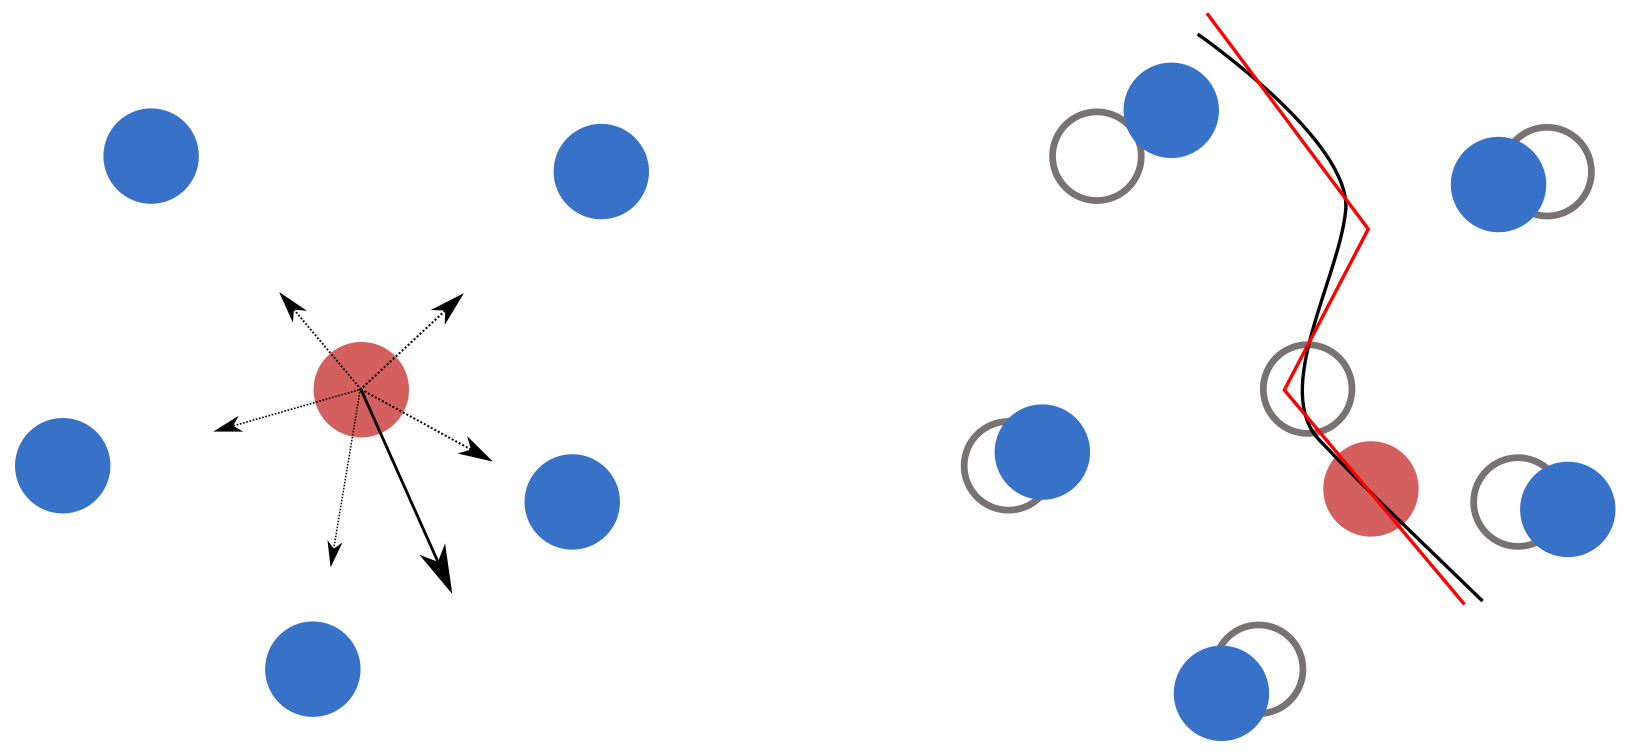
\includegraphics[width=0.8\textwidth]{chapter/main/theory/img/scheme_md.png}
			\caption{Schematische Darstellung der Trajektorienerstellung bei der klassischen
			Molekulardynamik mithilfe eines beliebigen iterativen Integrators. Im ersten Schritt
			(links) wird die auf das rote Teilchen wirkende Gesamtkraft bestimmt. Gleiches
			passiert auch für die anderen Teilchen. Im nächsten Schritt (rechts) werden nun alle
			Teilchen entsprechend der auf sie wirkenden Kräfte verschoben und bilden somit in
			guter Näherung die Trajektorie der jeweiligen Teilchen.
			\cite{sonntag2011computer}}
			\label{fig:scheme_md}
		\end{figure}

		Ein etabliertestes Modellpotential für klassische MD mit ungeladenen Teilchen ist das
		\emph{Lennard-Jones-Potential} (\emph{LJ})

		\begin{align}
			U^\text{LJ}(r) &= 4\epsilon \left[
				\left(\frac{\sigma}{r}\right)^{12}
				-
				\left(\frac{\sigma}{r}\right)^{6}
			\right]
			\label{eq:potential_lj}
		\end{align}

		mit der der Nullstelle $\sigma$ und der Tiefe der Potentialmulde $\epsilon$. Es hat sich
		deswegen etabliert, weil das Potential einerseits analytischer Natur und einfach
		differenzierbar ist, andererseits die Wechselwirkungen zwischen zwei Teilchen sehr gut
		abbildet. Es modelliert die schwache, aber langreichweitige Van-der-Waals-Bindung mit der
		London-Kraft $~ r^{-6}$ und das starke, aber kurzreichweitigere Pauli-Prinzip mit einem
		Repulsionsterm $\sim r^{-n}$, wobei aus praktischen Gründen oft $n=12$ gewählt wird. In
		Abbildung \ref{fig:potential_lj} ist zu erkennen, dass das Potential einerseits eine
		abrupte Abstoßung naher Teilchen bewirkt, andererseits für eine Anziehung weiter
		entfernter Teilchen sorgt.

		\begin{figure}[!ht]
			\centering
			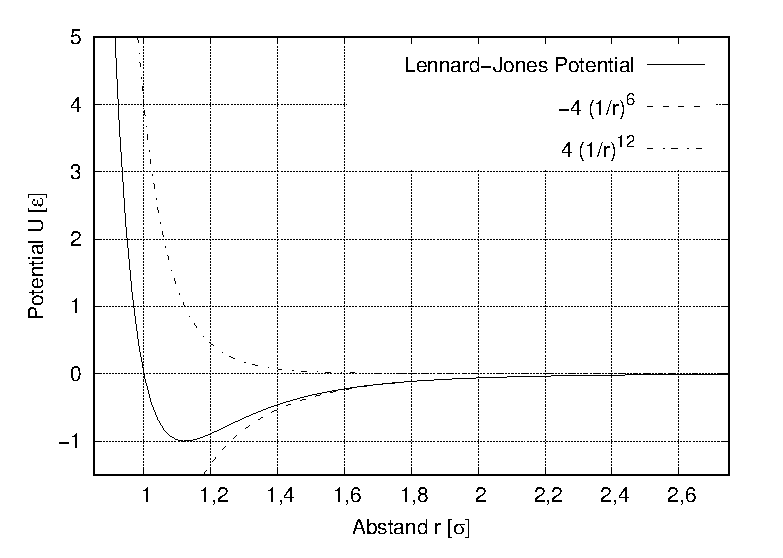
\includegraphics[width=0.8\textwidth]{chapter/main/theory/plt/lennard_jones.eps}
			\caption{Auftragung der Funktion in Gleichung \eqref{eq:potential_lj} in Einheiten
			der Parameter $\epsilon$ und $\sigma$}
			\label{fig:potential_lj}
		\end{figure}

		Die auf vom Teilchen $j$ auf das Teilchen $i$ wirkende Kraft
		\begin{align}
			\uvec{F}_{ij} &= -\nabla_i U^\text{LJ}\left(
				\left\|\uvec{x}_i - \uvec{x}_j\right\|
			\right)
		\end{align}
		ergibt sich durch explizites Einsetzen des Potentials und Bildung des negativen Gradienten.
		Das lediglich vom Abstand $r$ abhängige LJ-Potential ergibt also eine entlang des
		Richtungsvektors $\uvec{r}_{ij} = \uvec{x}_j - \uvec{x}_i$ wirkende Kraft

		\begin{align}
			F_{ij}(r) &= 24\epsilon \frac{\uvec{r}_{ij}}{r^2} \left[
				2\left(\frac{\sigma}{r}\right)^{12}
				-
				\left(\frac{\sigma}{r}\right)^{6}
			\right]
			\label{eq:force_lj}
			.
		\end{align}

		Da für jedes der $N$
		Teilchen $N-1$ Einzelkräfte berechnet werden müssen, skaliert die Anzahl der Berechnungen
		mit $N(N-1)$ ($\rightarrow N^2$ für große $N$). Durch Newtons drittes Gesetz
		$\uvec{F}_{ij} = -\uvec{F}_{ji}$ lässt sich die Anzahl der expliziten Kraftberechnungen
		halbieren, wobei das Skalierungsverhalten weiterhin quadratisch bleibt.

	\subsection{Reduzierte Einheiten}
	\todo[color=red]{Kapitel über reduzierte Einheiten schreiben}

	\subsection{Numerische Integration der Newtonschen Bewegungsgleichungen}
		Alle iterativen Verfahren zur numerischen Integration von Bewegungsgleichungen basieren
		im wesentlichen auf einer Taylorentwicklungen

		\begin{align}
			\uvec{x}_{n+1} &= \sum_{k=0}^\infty \frac{\uvec{x}^{(k)}_n}{k!} \dt^k
		\end{align}

		der Trajektorien um die Stelle $\dt = 0$. Hierbei bezeichnet $\uvec{x}^{(k)}$ die $k$-te
		Zeitableitung von $\uvec{x}$. Mithilfe der Diskretisierung des Zeitschritts \dt lässt sich von einem
		Integrationsschritt $n$ näherungsweise auf den nächsten $n+1$ schließen.

		Die wohl simpelste Methode der numerischen Integration ist das \emph{Euler-Verfahren}.
		Für dieses wird das Taylorpolynom ersten Grades der Trajektorie

		\begin{align}
			\uvec{x}_{n+1} &= \uvec{x}_n + \dot{\uvec{x}}_n \dt + \BigO\left(\dt^2\right)
		\end{align}

		verwendet und alle höheren Terme verworfen. Hierbei bezeichnet $\dot{\uvec{x}}$ die erste
		Ableitung von $x$ nach der Zeit, $\ddot{\uvec{x}}$ die zweite Ableitung, und so weiter.
		Das Problem, welches dem Euler-Verfahren innewohnt, ist die nicht-symplektische Natur.
		Somit kann die für ein mikrokanonisches Ensemble notwendige Forderung nach
		Energieerhaltung nicht erfüllt werden \cite{klein2013klassische}.

		Ein symplektischer Algorithmus ist der \emph{Verlet-Algorithmus}. Er entsteht durch zwei
		Taylorentwicklungen 4. Ordnung der Trajektorie wie in den Gleichungen
		\eqref{eq:verlet_taylor_fw} und \eqref{eq:verlet_taylor_bw}, wobei eine der Entwicklungen
		mit positivem Zeitschritt \dt und eine mit negativem Zeitschritt -\dt durchgeführt wird
		\cite{frenkel2001understanding}. Es gilt jeweils

		\begin{align}
			&&\uvec{x}_{n+1} &= \uvec{x}_n + \dot{\uvec{x}}\dt + \frac{1}{2}\ddot{\uvec{x}}\dt^2
				+ \frac{1}{3!}\dddot{\uvec{x}}_n\dt^3 + \BigO\left(\dt^4\right)
				\label{eq:verlet_taylor_fw} \\
			&\text{und}&
			\uvec{x}_{n-1} &= \uvec{x}_n - \dot{\uvec{x}}\dt + \frac{1}{2}\ddot{\uvec{x}}\dt^2
				- \frac{1}{3!}\dddot{\uvec{x}}_n\dt^3 + \BigO\left(\dt^4\right)
				\label{eq:verlet_taylor_bw}
				.
		\end{align}

		Durch Addition beider Taylorpolynome ergibt sich damit ein symplektischer Algorithmus

		\begin{align}
			\uvec{x}_{n+1} &= 2 \uvec{x}_n - \uvec{x}_{n-1} + \ddot{\uvec{x}}_n\dt^2
				+ \BigO\left(\dt^4\right) \label{eq:verlet},
		\end{align}

		der aufgrund seiner Abhängigkeit vom $n-1$-ten Wert nicht selbststartend ist.

		Wie auch in der für diese Arbeit genutzten Simulationssoftware \emph{IMD}
		\cite{stadler1997imd} wird jedoch für MD-Simulationen häufig der zum Verlet-Verfahren
		äquivalente \emph{Velocity-Verlet-Algorithmus}

		\begin{align}
			\uvec{x}_{n+1} &= \uvec{x}_n + \dot{\uvec{x}}\dt
				+ \frac{1}{2}\ddot{\uvec{x}}\dt^2 + \BigO\left(\dt^4\right) \nonumber\\
			\dot{\uvec{x}}_{n+1} &= \dot{\uvec{x}}_n + \frac{\ddot{\uvec{x}}_n +
				\ddot{\uvec{x}}_{n+1}}{2}\dt + \BigO\left(\dt^2\right)
				\label{eq:velocity_verlet}
		\end{align}

		verwendet. Durch die Äquivalenz der beiden Algorithmen bleibt die symplektische Natur
		erhalten, jedoch ist der Algorithmus nun geschwindigkeitsabhängig. In der klassischen MD
		ist dies jedoch kein Problem, da die Geschwindigkeiten ohnehin von Interesse für manche
		Größen (wie beispielsweise die Temperatur des Systems) sind. Zudem ist er selbststartend,
		wodurch einzelne Anfangswerte ausreichen und auch keine Anfangswertepaare durch
		Integration mit einem anderen Integrator erzeugt werden müssen.

	\subsection{Erweiterung von IMD} % Implementierung des Lasers
		Bestrahlt man ein Material mit einem Laser, so regen die Photonen die Elektronen im
		Material an. Nur eine bestimmte Anzahl an Elektronen existiert, die in der infinitesimalen
		Eindringtiefe $\dx$ genau die Energie der eingestrahlten Photonen aufnehmen können. Da die
		Anzahl der Photonen proportional zur Intensität des Lasers ist, sinkt die
		Absorptionswahrscheinlichkeit mit sinkender Intensität. Dieses Verhalten wird mit dem
		\emph{Lamber-Beer'schen} Gesetz

		\begin{align}
			-\frac{\dx[I]}{\dx[x]} &= \mu I(x)
			&\Rightarrow&&
			I(x) &= I(0) \cdot \exp\left(-\mu x\right)
		\end{align}

		beschrieben. Die Anzahl der angeregten Elektronen nimmt also exponentiell mit der
		Eindringtiefe des Lasers ab \cite{klein2013klassische}. Das System wird durch die Anregung
		der Elektronen in einen Zustand versetzt, der ich vom Gleichgewichtszustand unterscheidet.
		Das Elektronensystem, welches örtlich ungleichmäßig angeregt wurde, strebt nun gemäß der
		thermodynamischen Gesetze wieder zum Gleichgewichtszustand. Diese durch
		Elektron-Elektron-Stoßprozesse stattfindende Diffusion der Elektronentemperatur heißt
		\emph{Thermalisierung}. Durch Elektron-Phonon-Kopplung überträgt sich die Energie des
		Elektronensystems auf das Gitter, was jedoch auf einem wesentlich größeren Zeitintervall
		geschieht als die Thermalisierung. Da in der MD jedoch einzelne Atome und keine Elektronen
		modelliert werden, bedarf es des sogenannten \emph{Reskalierungsmodells} (\emph{RM}).
		Da sich die Thermalisierung in einer zeitlich wesentlich kleineren Größenordnung abspielt
		als die der Simulationsschrittweite, kann das Aufheizen des Materials als örtlich begrenzte
		instantane Erhöhung der kinetischen Energie der Teilchen modelliert werden
		\cite{klein2013klassische}.

		Nach dem Äquipartitionstheorem

		\begin{align}
			\left\langle E_\text{kin} \right\rangle &= \frac{f}{2} k_\text{B} T
				\label{eq:equipartition}
		\end{align}

		ist hierbei die mittlere kinetische Energie $\left\langle E_\text{kin} \right\rangle$
		proportional zur Temperatur $T$, wobei $f$ die Anzahl der Freiheitsgrade und
		$k_\text{B}$ die Boltzmannkonstante ist.

		Die wohl direkteste Implementierung des Aufheizens durch einen Laser ist das Skalieren
		der Teilchengeschwindigkeiten gemäß eines durch Gleichung \eqref{eq:equipartition}
		geforderten Faktors für die Geschwindigkeiten. Sei nun die gewollte Energieänderung
		$\dx[E]$. Mit $E_\text{kin} \sim \dot{\uvec{x}}^2$ folgt also für den Faktor mit
		$\dot{\uvec{x}}(t + \dt) = a\dot{\uvec{x}}(t)$

		\begin{align}
			a^2 &= \frac{E_\text{kin}(t + \dt)}{E_\text{kin}(t)}
			&\Rightarrow&&
			a &= \sqrt{\frac{E_\text{kin}(t) + \dx[E]}{E_\text{kin}(t)}}
				= \sqrt{1 + \frac{\dx[E]}{E_\text{kin}(t)}}
			.
			\label{eq:factor}
		\end{align}

		Da $E_\text{kin}(t)$ durch Summation aller Geschwindigkeitsquadrate einfach bestimmt
		werden kann, bleibt als unbekannte die gewünschte Energieeinbringung $\dx[E]$. Um diese
		zu bestimmen wird ein gaußförmiges Intensitätsprofil in der Form

		\begin{align}
			I(r) &= I_0 \exp\left(-\frac{r^2}{2\sigma}\right) \label{eq:gauss_profile}
		\end{align}

		mit der Varianz der Gauß-Funktion $\sigma$ angenommen. Abbildung \ref{fig:gauss} zeigt
		eine normierte Gaußfunktion. Aufgrund der Normierung ändern sich mit der Variation von
		$\sigma$ die Breite und die Höhe antiproportional zueinander.

		\begin{figure}[!ht]
			\centering
			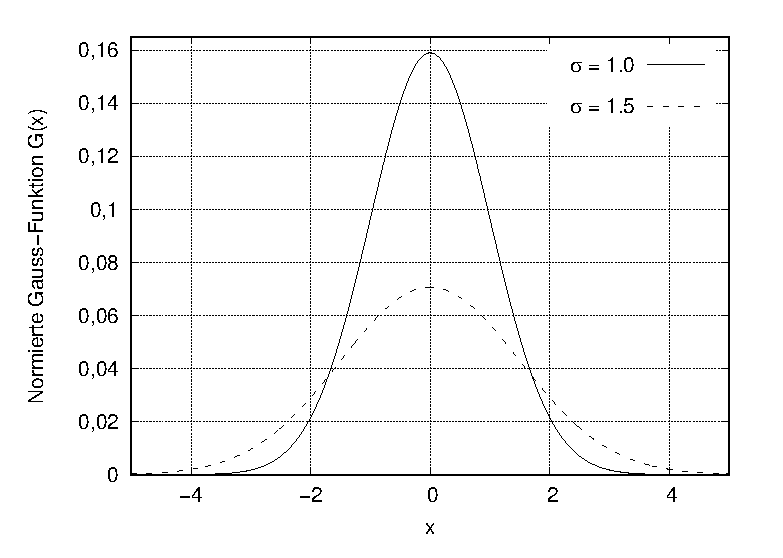
\includegraphics[width=0.8\textwidth]{chapter/main/theory/plt/gauss.eps}
			\caption{Eine normierte Gauß-Funktion wird mit abnehmender Breite höher und
			umgekehrt für variierendes $\sigma$}
			\label{fig:gauss}
		\end{figure}

		Nach Gleichung \eqref{eq:gauss_profile} ist das Intensitätsprofil nur vom Abstand $r$
		zur Strahlachse abhängig. Für einen Laser in $z$-Richtung ist $r^2 = x^2 + y^2$. Eine
		Integration entlang der Ebene senkrecht zur Strahlrichtung muss die Gesamtleistung
		$P_\text{Ges}$ des Lasers ergeben, sodass der Zusammenhang

		\begin{align}
			P_\text{Ges} &= \int_{\mathbb{R}^2} I(r) \dx\dx[y]
				= I_0 \int_0^{2\pi} \dx[\theta] \int_0^\infty \exp\left(-a r^2\right) \dx[r]
		\end{align}

		gilt. Drückt man die Varianz nun als Halbwertsbreite $\fwhm = 2\sqrt{2 \ln2}\sigma$ aus, so
		ergibt sich für die maximale Intensität

		\begin{align}
			I_0 &= \frac{P_\text{Ges}}{\pi} \frac{4\ln2}{\fwhm^2}
			.
		\end{align}

		Da in der Herleitung bisher noch keine Intensitätsabschwächung nach dem
		\emph{Lambert-Beer-Gesetz} mit der Absorption $\mu$ erfolgt ist, wird die Intensität mit
		dem entsprechenden Faktor multipliziert. Ebenso wird direkt der Reflexionskoeffizient
		$R$ mit eingebunden.

		\begin{align}
			I(x,y,z) &= \exp\left(-\mu z\right) \cdot (1-R) \cdot I(x,y)
			\label{eq:intensity}
		\end{align}

		Da allerdings nicht die Intensität direkt notwendig ist, sondern die Änderung der
		kinetischen Energie und damit der Geschwindigkeiten nach Gleichung \eqref{eq:factor}, muss
		die diskrete Energieänderung $\dx[E]$ berechnet werden. Dazu bedarf es einer Betrachtung
		der Größen pro diskreter Volumeneinheit $\dx[V]$ und pro Zeitschritt $\dt$

		\begin{align}
			\dx[I] &= \frac{\dx[E]}{\dx[A]\cdot\dt}
			&\Leftrightarrow&&
			\dx[E] &= \dx[I] \cdot \dx[A] \cdot \dt
			.
		\end{align}

		Erweitern mit $\dx[z]/\dx[z]$ führt nun auf die Form

		\begin{align}
			\dx[E] &= \frac{\dx[I]}{\dx[z]} \cdot \dx[z] \cdot \dx[A] \cdot \dt
				= \frac{\dx[I]}{\dx[z]} \cdot \dx[V] \cdot \dt
			.
			\label{eq:energy_diff_1}
		\end{align}

		Zwar ist $\dx[I]/\dx[z]$ ein Differenzenquotient, im diskreten Kontext aber kommt diesem
		die gleiche Bedeutung wie die Ableitung $\partial_z I$ zu. Diese ist durch Gleichung
		\eqref{eq:intensity} bekannt, sodass der Gesamtausdruck für die Energieänderung nun

		\begin{align}
			\dx[E] &= (1-R) \cdot \mu \cdot \exp\left(-\mu z\right)
				\cdot \frac{P_\text{Ges}}{\pi \sigma_\text{sc}^2}
				\cdot \exp\left(-\frac{x^2 + y^2}{\sigma_\text{sc}^2}\right)
				\cdot \dx[V] \cdot \dt
		\end{align}

		lautet. Zu beachten ist, dass $\sigma_\text{sc}^2 = 2\sigma^2 = \fwhm^2/(4\ln2)$ nicht die
		Varianz ist, sondern nur der übersichtlicheren Darstellung dient.

	\subsection{Verwendete Näherungen}
		%\todo[color=red]{Implementierung des Lasers: Lambert-Beer-Gesetz wie es implementiert ist eigtl nur für ebene Oberflächen gültig.}
		\subsubsection{Lambert-Beer'sches Gesetz}
		Eine Näherung, die aus Gründen der einfacheren Implementierung und der besseren
		Rechenleistung sinnvoll ist, ist eine vereinfachte Anwendung des Lambert-Beer'schen
		Gesetzes. Während bei diesem Gesetz eigentlich die Länge betrachtet wird, während der sich
		die elektromagnetischen Wellen tatsächlich im Medium befinden, wird hier für den Eintritt
		der Absorption ein fixer $z$-Wert angenommen. Dies hat den Grund, dass eine Absorption
		nach exakten Maßstäben nur durch eine Diskretisierung des Lasers in kleinere Unterstrahlen
		und eine darauf aufbauende Strahlverfolgung (\emph{Raytracing}) möglich wäre. Dies ist
		jedoch sehr rechenintensiv und müsste zudem nach jedem Simulationsschritt wiederholt
		werden. Weil diese Näherung für Geometrien mit in $z$-Richtung homogener Atomverteilung
		und gerader Oberkante (zum Beispiel quader- oder zylinderförmige Objekte) exakt ist, kann
		sie als annehmbare Näherung für kugelförmige Anordnungen, wie sie hier verwendet werden,
		gesehen werden. Zwar führt dies zu einer Änderungen in den Einzeltrajektorien, jedoch ist
		eine Änderung der makroskopischen Eigenschaften nicht zu erwarten, da die Dynamik des
		System näherungsweise gleich bleibt.

		\todo[color=red]{Kurzes Kapitel darüber warum Aluminium bzw über Alu an sich. zB AluSi10Mg
		enthält nach DIN EN 1706 ca. 90 \% Alu}
		%\todo[color=red]{Kleinere Skala und größere Gravitation mithilfe von \cite{glosli2007extending} motivieren.}
		\subsubsection{Änderungen der Größenordnungen}
		Für die Simulationen werden im Folgenden die Größenordnungen kleiner skaliert. Während die
		Partikelgröße der Pulverpartikel beim SLM-Verfahren üblicherweise im Bereich von wenigen
		Mikrometern \cite{hajnys2020research} was mit den bisher zur Verfügung stehenden
		Rechenleistungen nur schwer zu schaffen ist \cite{eckhardt2013scientists}. Aus diesem
		Grund wird eine Pulverpartikelgröße in der Größenordnung der hunderten \AA ngström
		angenommen. Die Einführung dieser Skalierungsfaktoren führt ebenfalls zu einer Änderung
		der Einheiten. Motiviert wird dies wird durch eine Veröffentlichung von Glosli et al.
		Diese Forschungsgruppe hat die Kelvin-Helmholtz-Instabilität bei verhältnismäßig kleiner
		Teilchenzahl als Ergebnis ihrer Simulation nachweisen können. Weil eben diese Instabilität
		stark von ihren Anfangswerten abhängt, kann das Auftreten dieser als Motivation verstanden
		werden den hier zu simuliernden Sachverhalt ebenfalls auf kleinere Maßstäbe zu schrumpfen,
		da hier im Wesentlichen ebenfalls das Verhalten von Fluiden von Interesse ist
		\cite{glosli2007extending}. Wie in dieser Veröffentlichung muss hier als Ausgleich dazu
		ebenfalls die Gravitation erhöht werden.

	%\subsection{Besonderheiten bei der Simulationssoftware IMD}
